\documentclass[leqno]{article}
\usepackage[utf8]{inputenc}
\usepackage[T1]{fontenc}
\usepackage{amsfonts}
%\usepackage{fourier}
%\usepackage{heuristica}
\usepackage{enumerate}
\author{Colin Roberts}
\title{MATH 571, Homework 10}
\usepackage[left=3cm,right=3cm,top=3cm,bottom=3cm]{geometry}
\usepackage{amsmath}
\usepackage[thmmarks, amsmath, thref]{ntheorem}
%\usepackage{kbordermatrix}
\usepackage{mathtools}
\usepackage{color}
\usepackage{hyperref}
\usepackage{tikz-cd}

\theoremstyle{nonumberplain}
\theoremheaderfont{\itshape}
\theorembodyfont{\upshape:}
\theoremseparator{.}
\theoremsymbol{\ensuremath{\square}}
\newtheorem{proof}{Proof}
\theoremsymbol{\ensuremath{\square}}
\newtheorem{lemma}{Lemma}
\theoremsymbol{\ensuremath{\blacksquare}}
\newtheorem{solution}{Solution}
\theoremseparator{. ---}
\theoremsymbol{\mbox{\texttt{;o)}}}
\newtheorem{varsol}{Solution (variant)}

\newcommand{\id}{\mathrm{Id}}
\newcommand{\im}{\mathrm{im}}
\newcommand{\R}{\mathbb{R}}
\newcommand{\N}{\mathbb{N}}
\newcommand{\Z}{\mathbb{Z}}

\begin{document}
\maketitle
\begin{large}
\begin{center}
Solutions
\end{center}
\end{large}

%%%%%%%%%%%%%%%%%%%%%%%%%%%%%%%%%%%%%%%%%%%%%%%%%%%%%%%%%%%%%%%%%%%%%%%%%%%%%%%%%%%%%%%%%%%%%%%%%%%%%%%%%%%%%%%%%%%%%
%%%%%%%%%%%%%%%%%%%%%%%%%PROBLEM%%%%%%%%%%%%%%%%%%%%%%%%%%%%%%%%%%%%%%%%%%%%%%%%%%%%%%%%%%%%%%%%%%%%%%%%%%%%%%%%%%%%%%%%%%%%%%%%%%%%%%%%%%%%%%%%%%%%%%%%%%%%%%%%%%%%%%%%%%%%%%%%%%%%%%%%%%%%%%%%%%%%%%%%%%%%%%%%%%%%%%%%%%%%%%%%%%%%%%%%%%

\noindent\textbf{Problem 1.} 
Compute the 0-, 1-, and 2-dimensional simplicial cohomology groups of the projective plane $\R P^2$ using $\Z$ coefficients, and using the $\Delta$-complex structure on page 102 of Hatcher:
\begin{center}
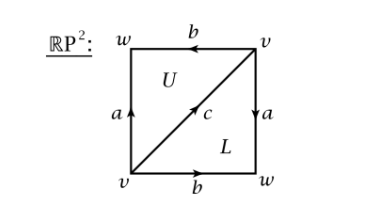
\includegraphics[width=2in]{RP2Delta.png}
\end{center}


\begin{proof}
Let $X$ denote $\R P^2$.  Then we have the following:
\begin{align*}
&\Delta^0(X;\Z) = \hom (\Delta_0 (X);\Z) = \hom(\Z^{\oplus 2};\Z) \cong \Z^2 \quad \textrm{generated by $v^*$ and $w^*$}\\
&\Delta^1(X;\Z) = \hom (\Delta_1 (X);\Z) = \hom(\Z^{\oplus 3};\Z) \cong \Z^3 \quad \textrm{generated by $a^*$, $b^*$ and $c^*$}\\
&\Delta^2(X;\Z) = \hom (\Delta_2 (X);\Z) = \hom(\Z^{\oplus 2};\Z) \cong \Z^2 \quad \textrm{generated by $U^*$ and $L^*$}\\
&\Delta^3(X;\Z) = \hom (\Delta_3 (X);\Z) = \hom(0;\Z)=0.
\end{align*}
Now we compute the image and kernel of $\delta^0$.
\begin{align*}
&(\delta^0 v^*)(a)=v^*(\partial a)=v^*(w-v)=-1\\
&(\delta^0 v^*)(b)=v^*(\partial a)=v^*(w-v)=-1\\
&(\delta^0 v^*)(c)=v^*(\partial a)=v^*(v-v)=0\\
& \implies \delta^0 v^* = -a^*-b^*\\
&(\delta^0 w^*)(a)=w^*(\partial a)=w^*(w-v)=1\\
&(\delta^0 w^*)(a)=w^*(\partial a)=w^*(w-v)=1\\
&(\delta^0 w^*)(a)=w^*(\partial a)=w^*(w-v)=0\\
& \implies \delta^0 w^* = a^*+b^*.\\
\end{align*}
Thus $\im \delta^0 \cong \Z$ and is generated by $\{a^*+b^*\}$ and $\ker\delta^0 \cong \Z$ is generated by $\{v^*+w^*\}$. Hence we have
\[
H^0(X;\Z)=\ker \delta^0 \cong \Z.
\]
\end{proof}
We repeat the process for $\delta^1$.
\begin{align*}
&(\delta^1 a^*)(U)=a^*(\partial U)=a^*(a-b-c)=1\\
&(\delta^1 a^*)(L)=a^*(\partial L)=a^*(a-b+c)=1\\
& \implies \delta^1 a^* = U^*+L^*\\
&(\delta^1 b^*)(U)=b^*(\partial U)=b^*(a-b-c)=-1\\
&(\delta^1 b^*)(L)=b^*(\partial L)=b^*(a-b+c)=-1\\
& \implies \delta^1 b^* = -U^*-L^*\\
&(\delta^1 c^*)(U)=c^*(\partial U)=c^*(a-b-c)=-1\\
&(\delta^1 c^*)(L)=c^*(\partial L)=c^*(a-b+c)=1\\
& \implies \delta^1 c^* = -U^*+L^*.\\
\end{align*}
Thus $\im \delta^1 \cong \Z^2$ and is generated by $\{U^*+L^*,2U^*\}$ and $\ker\delta^1 \cong \Z$ is generated by $\{a^*+b^*\}$. Since $\ker \delta^1$ is generated by $\{a^*+b^*\}$ and $\im \delta^0$ is generated by $\{a^*+b^*\}$ we have
\[
H^1(X;\Z)\cong 0.
\]
Now $\delta^2 =0$ since there are no $3$-simplicies. So since $\ker \delta^2$ is generated by $\{U^*+L^*,U^*\}$ and $\im \delta^1$ is generated by $\{U^*+L^*,2U^*\}$ we have that
\[
H^2(X;\Z)\cong \Z/2\Z.
\]

\vspace*{1cm}


\noindent\textbf{Problem 2.} 
Confirm that your answer to \# 1 agrees with Corollary 3.3 on page 196 of our book (and with our computation of the simplicial homology groups of the projective plane, for example in our notes on 2/16/18 or in Example 2.4 of Hatcher).\\

\noindent \emph{Remark: The point of this problem is to make sure you are aware of Corollary 3.3 (and perhaps pique your curiosity), even if you do not have an understanding of why Corollary 3.3 is true.}

\begin{proof}
From \# 1 we have that
\begin{align*}
H^i(\R P^2 ; \Z)= 
\begin{cases}
\Z & i=0\\
0 & i=1\\
\Z/2\Z & i=2\\
\end{cases}
\end{align*}
We also know that 
\begin{align*}
H_i(\R P^2 ; \Z)= 
\begin{cases}
\Z & i=0\\
\Z/2\Z & i=1\\
0 & i=2.
\end{cases}
\end{align*}
\end{proof}
Following the corollary, we find that
\[
H_0(\R P^2; \Z)\cong \Z,
\]
meaning there is no torsion (i.e., $T_0=0$) and 
\[
H^0(\R P^2 ; \Z) \cong \Z.
\]
Next, look at
\[
H_1(\R P^2; \Z) \cong \Z/2\Z,
\]
where there is \emph{only} a torsion group (i.e., $T_1=\Z/2\Z$).  Then
\[
H^1(\R P^2; \Z) \cong (H_1/T_1)\oplus T_{0} \cong (\Z/2\Z)/(\Z/2\Z)\oplus 0 \cong 0.
\]
Then, we finally have that
\[
H_2(\R P^2; \Z) \cong 0,
\]
but because $T_1=\Z/2\Z$ we have that
\[
H^2(\R P^2; \Z) \cong (H_2/T_2) \oplus T_1 \cong \Z/2\Z.
\]
So the corollary gives us the correct answer! Woohoo!


\vspace*{1cm}


\noindent\textbf{Problem 3.} 
Redo \# 1, except now with $\Z/2\Z$ coefficients.

\begin{proof}
Let $X=\R P^2$ and also note that $\hom(\Z;\Z/2\Z)\cong \Z/2\Z$.  Then we will use results from Problem 1 to make this computation shorter.  We have that $\im \delta^0$ is generated by $a^*+b^*$ and $\ker \delta^0$ is generated by $v^*+w^*$. This gives
\[
H^0(X;\Z/2\Z)\cong \Z/2\Z.
\]
Then we have that $\ker \delta^1$ is generated by $a^*+b^*$ from computations in Problem 1, but, in addition, is also generated by $a^*+c^*$ since 
\[
\delta^1 (a^*+c^*)=2L^*=0.
\]
Then
\[
H^1(X;\Z/2\Z) \cong \Z/2\Z.
\]
We also have that $\im \delta^1$ is generated only by $U^*+L^*$ since in our calculation before we had the other generator $2U^*$ which is identically 0 in $\Z/2\Z$. Then again $\delta^2=0$ so $\ker \delta^2$ is generated by $U^*+L^*$ and $U^*$. So we have
\[
H^2(X;\Z/2\Z)\cong \Z/2\Z.
\]
\end{proof}

\vspace*{1cm}


\noindent\textbf{Problem 4.} 
Redo \# 1, except now with $\Z/3\Z$ coefficients.

\begin{proof}
Again, letting $X=\R P^2$ and note that $\hom(\Z;\Z/3\Z) \cong \Z/3\Z$. We have that $\ker \delta^0$ is generated by $v^*+w^*$ which gives
\[
H^0(X; \Z/3\Z) \cong \Z/3\Z.
\]
We also have that $\im \delta^0$ is generated by $a^*+b^*$.  Also, $\ker \delta^1$ is generated by $a^*+b^*$ and we don't have the extra generator as we did in Problem 3 since we are now working over $\Z/3\Z$. This gives
\[
H^1(X;\Z/3\Z)\cong 0.
\]
So $\im \delta^1$ is generated by $U^*$ and $L^*$ and $\ker \delta^2$ is generated by $-U^*+L^*$ and $U^*+L^*$. Note that $2(U^*+L^*)+(-U^*+L^*)=U^*$ and $-2(-U^*+L^*)+2(U^*+L^*)=L^*$ and so 
\[
H^2(X;\Z/3\Z)\cong 0.
\]

\end{proof}

\end{document}



